\chapter{Validation and Evaluation}
\label{chap:validationevaluation}

%In order to ensure that  we fulfill the requirements listed in Chapter \ref{chap:spec}, in this chapter we provide a testing of the main components we implemented and we describe how we initialize the different testing scenarios. In Section \ref{sec:multitenanttest} we provide three different testing scenarios, one per extended \ac{BC}, and we monitor both incoming and outgoing messages to and from the \ac{ESB}.

In this chapter we provide the validation, and evaluation of the system. We must ensure that the requirements specified in Chapter \ref{chap:spec} are fulfilled in the design and implementation phases. In Section \ref{sec:deploymentandinit} we describe the steps which should be followed to initialize the system, and the testing scenarios. After the initialization we execute the test cases in Section \ref{sec:validation}, and monitor the incoming requests to ServiceMix-mt, and the outgoing requests to the backend Cloud data store. Due to the extensions implemented on the \ac{ESB}, we evaluate in Section \ref{sec:evaluation} its behavior, and the impact that our modifications have on the original ServiceMix-mt.

\section{Deployment and Initialization}
\label{sec:deploymentandinit}

The validation and evaluation of the prototype must close to the motivating scenario. Therefore, we must perform the testing of the prototype in a Cloud environment. We are provided with a VM image in the FlexiScale Cloud infrastructure \cite{flexiscale}, which runs the operative system Ubuntu 10.04 64 bits. The following components are deployed in the VM:
\begin{itemize}
	\item ServiceMix-mt 4.3.0: the multi-tenant aware ServiceMix 4.3.0. In addition to the \ac{OSGi} bundles, \ac{JBI} \ac{SA}s, and JBIMulti2 shared library \cite{JBIMulti2Man}, in its deploy folder we store the \ac{JBI} ServiceMix Registry, CDASMix MySQL Proxy, and the CamelJDBCCdasmix \ac{OSGi} bundles for deployment. 
	\item JOnAS 5.2.2: the Java application server which hosts the JBIMulti2 application. 
	\item MySQL database 5.1: MySQL database system for performing evaluation and validation of the prototype with a local database instance.
	\item PostgreSQL 9.1.1:  PostgreSQL database system which stores the tenant-aware configuration data in the Service Registry, Configuration Registry, and Tenant Registry. 
\end{itemize} 

For more information about the deployment, and initialization of the ServiceMix-mt and JBIMulti2 please refer to the document "Manual for the JBIMulti2 Implementation" \cite{JBIMulti2Man}. On the other hand, we utilize de following off-premise instances:
\begin{itemize}
	\item Amazon RDS db.m1.micro instance: MySQL 5.5 database system hosted in the Amazon RDS Cloud infrastructure. 
	\item Amazon DynamoDB table: \ac{NoSQL} key-value database for storing objects in the created tables. 
	\item Google Cloud Storage: \ac{NoSQL} key-value database for storing buckets and objects.
\end{itemize} 

We must maximize the approximation of the testing and evaluation scenarios with the motivating scenario. Therefore, we perform the testing cases from a local machine in the University of Stuttgart network infrastructure, in order to simulate the access to the data from an on-premise data access layer. Communication with the JBIMulti2 application for tenant configuration, and deployment of \ac{SA}s is established using soapUI 3.6. Communication with the MySQL endpoint in ServiceMix-mt is established using the MySQL Connector/J 5.1.22, while for the different tenant-aware \ac{HTTP} endpoints we use the Java libraries provided by the Cloud data store providers. 
\section{Validation}
\label{sec:validation}

In this section we provide an overview of the messages, and programs used for the validation of the prototype. The transmission of the following message samples requires the system to be started, and the operations until the deployment of the tenant operator's \ac{SA} to be executed. These messages are provided in a soapUI test suite shipped with the prototype. From the moment when the tenant deploys the \ac{SA}, the configuration of the frontend and backend data stores can be associated to it. The data store configuration is done through the execution of operations which are accessible through a Web service interface. Therefore, either the \term{Cloud Data Migration Tool}, or the tenant can configure their database connections through the \ac{ESB} to the backend Cloud data store where his data is migrated to.
 
\lstinputlisting[label={lst:testaddds},caption={[Add Source and Target Data Source Sample Request]Add Source and Target \ac{SQL} Data Source \ac{SOAP} over \ac{HTTP} sample request.},style=xml]{./gfx/addds.xml}

The message described in Listing \ref{lst:testaddds} contains the needed information for registering and providing access to the tenant operator A in the MySQL CDASMix Proxy, and connecting with an \ac{SQL} database system in a backend Cloud data store. The tenant operator must authenticate with JBIMulti2 in order to register the connection meta-data, e.g. protocol, URL, database type, access credentials, etc. In Listing \ref{lst:testaddds} the tenant operator A, which is a user of the tenant Taxi Company, registers for the endpoint configuration described in the \term{servicemix.cdasmix.jbi.camelSA} a connection with a MySQL 5.1.3 database system instance in the Amazon RDS infrastructure. When more than one target database system wants to be attached to an existing source data source registered in the system, this provides the \term{AttachTargetDataSource} operation, which has as pre-condition the existence of the specified source data source.

\lstinputlisting[label={lst:testaddmis},caption={[Add Source and Target Main Information Structure Sample Request]Add Source and Target  \ac{SQL} Main Information Structure \ac{SOAP} over \ac{HTTP} sample request.},style=xml]{./gfx/addmaininfosql.xml}

When the source and target data source configuration are registered, the tenant operator (or through the \term{Cloud Data Migration Tool}) can register the storage structure meta-data of his database. For example, for a MySQL database system instance in Amazon RDS, the tenant operator must provide the tables' name (see Listing \ref{lst:testaddmis}), or for a bucket stored in a backend Google Cloud Storage container the tenant must provide the bucket identifier.

\lstinputlisting[label={lst:testaddsis},caption={[Add Source and Target Secondary Information Structure Sample Request]Add Source and Target \ac{NoSQL} Secondary Information Structure \ac{SOAP} over \ac{HTTP} sample request.},style=xml]{./gfx/addsecinfonosql.xml}

Registration of secondary information structure meta-data applies only for \ac{NoSQL} databases. The message described in Listing \ref{lst:testaddsis} contains the registration meta-data for an item stored in a table in the Amazon DynamoDB infrastructure. 

After the migrated data's meta-data is registered in the system, the tenant operator can access transparently the system using the standardized database access protocols, e.g. MySQL for the MySQL database system, and \ac{HTTP} for \ac{NoSQL} databases. 

\lstinputlisting[label={lst:testjdbc},caption={[Test Retrieving Information from Backend and Local Data Store]Retrieve data via \ac{JDBC} and MySQL protocol migrated to a backend Cloud data store, or local database system.},style=xml]{./gfx/testclient.java}

In Listing \ref{lst:testjdbc} we provide part of a Java program which connects via the MySQL Connector/J native driver with the MySQL CDASMix Proxy component on the port 3311. The options attached to the connection URL must be set as in the provided code in order to increase the performance of the communication, e.g. multi-querying for multiple queries in one statement, cache server configuration in order not to request the server configuration data per request, etc. In the MySQL request in Listing \ref{lst:testjdbc}, the tenant operator authenticates with the tenant and user UUID, and its password. Password is read in the system, but it is not compared in the authentication process, as the CDASMix MySQL proxy does not implement the hashing mechanisms of a MySQL server. After successful authentication, it executes a query which contains multiple queries in the same request. Each query is processed independently in the system when retrieving information from the different backend database systems, e.g. the \term{customer} table is stored in Amazon RDS, while mainInfoTest4 and mainInfoTest1 are stored in the local MySQL database system. The response is received as a single statement which contains n result sets, one for each query in the multi-query. 

\FloatBarrier
\chapter{Performance Evaluation}
\label{chap:performanceevaluation}

In the following sections we provide the requirements which should fulfill the performance evaluation of the \ac{ESB} solution we extend for multi-tenancy awareness. For this purpose, we extend a load generator developed by AndroitLogic to enable it with tenant-aware messaging \cite{androit2012}. Finally, we provide an overview of the components and systems involved in the different scenarios of the evaluation, and the design approach and implementation of the extension.

\section{Specification}
\label{sec:evaluationspecification}



\subsection{Evaluation Requirements}
\label{sec:evalrequirements}

% different message size, reduce loose couple being able to specify different types of messages
% invoke the endpoints with concurrent users and invoke endpoints concurrently
% be able to set the number of concurrent users and concurrent endpoints to invoke at the same time
% include multi-tenancy awareness in the benchmark for the different scenarios
% structured data as the output for analysis, for throughput and response time for the different messages requests for the different endpoints
% has to be done on top of the androitbenchmark, so that we can reuse and extend their benchmark
% system measurements of cpu and memory in structured data. also the measurement of the heap size (real memory consumtion) in the process
% monitoring of number of outgoing requests and incoming requests into the backend service, wireshark

In this student thesis we provide a performance analysis on the integration of the multi-tenant aware approaches in ServiceMix and measure the impact on the performance of the extended prototype. For this purpose, we need to fix which measurements we use for the evaluation. The driver should perform the following measurements: response time (measured in milliseconds) and throughput (measured in number of messages sent per second) respect to a backend service, and CPU and memory usage of the system hosting the instance of ServiceMix. The evaluation has to be done in different scenarios, each of them sending different messages number and sizes, for different multi-tenant and non multi-tenant aware endpoint configurations, as described in Table \ref{tab:evaluation} \cite{EvalESB}.

\begin{table}[htbp]
\centering
\begin{tabular}{llll}

	\toprule
	 Number of Endpoints 		& Messages Size	& ServiceMix Instances		& Multi-tenancy awareness 		\\
	 \midrule
	 
	 1 						& 0.5 / 1 KB 		& 1						& mt and non-mt									\\
	  						& 				& 2						& non-mt											\\
	 2 						& 0.5 / 1 KB 		& 1						& mt and non-mt									\\
	  						& 				& 2						& non-mt											\\
	 4 						& 0.5 / 1 KB 		& 1						& mt and non-mt									\\
	  						& 				& 2						& non-mt											\\
	 10 						& 0.5 / 1 KB 		& 1						& mt and non-mt									\\
	  						& 				& 2						& non-mt											\\														
	 
	\bottomrule
\end{tabular}
\caption[ServiceMix evaluation performance scenarios]{Specification of the different scenarios to be evaluated. In both multi-tenant and non multi-tenant aware evaluations, one user per endpoint / tenant is configured. \\ \term{Legend: mt (multi-tenant aware), non-mt (non multi-tenant aware)}}
	\label{tab:evaluation}
\end{table}

AndroitLogic has developed a performance analysis driver which fulfills most of the above requirements in different scenarios \cite{androit2012}. In our evaluation, we extend the Direct Proxy scenario from the AndroitLogic  \ac{ESB} Performance benchmark \cite{androit2012}. However, it doesn't achieve one of the main requirements of this student thesis: multi-tenant aware messaging and concurrent invocation between endpoints. Those two requirements should be included in an extended version of the primitive driver. Furthermore, the extension should be utilized with different \ac{ESB} solutions and must be user-friendly configurable for the different scenarios. The output of the driver measurements should be analyzed, therefore the output data must be in structured format. 

\subsection{Evaluation Overview}
\label{sec:evaluationoverview}

% main picture of the overview of the system for evaluating the esb and explain it with detais of the hardware setup of the vm
% describe a little bit the scenarios that were fixed
% 
In the Section \ref{sec:requirements} we have described the requirements that the evaluation should fulfill and the needed modifications in the utilized benchmark. As exposed in Figure \ref{fig:evaluationoverview}, the evaluation is conformed by three main independent systems. We must ensure, for analyzable purposes, that we approximate as much as possible to a Web service standard real scenario: service requester invokes a backend service and both request and response are routed through the network. In our evaluation we must utilize the \ac{ESB} as a mediator between the service requester and provider. In the first system (VM0), both service requestor and provider are deployed. The communication measurements are taken in two different components: throughput and response time in the AndroitLogic driver, while the number of incoming and outgoing requests, as well as the visualization of the messages, have to be monitored in an independent monitoring component. 

In the second and third systems (VM1 and VM2 respectively) one instance of ServiceMix is deployed for routing the messages between the AndroitLogic driver and the backend service. A monitor component must perform the counting of the incomming and outgoing requests to and from the \ac{ESB}, and a system monitor component should measure the \ac{ESB}'s resources consumption. The connection between the components in VM0 and VM2 is represented with a dashed line, because the VM2 is only use for non multi-tenant aware scenarios. Similarly, we have connected the components in VM0 with the components in VM1 with a continuos line, because this connection is used in both multi-tenant and non multi-tenant aware scenarios. 

The JBIMulti2 application is used for deployment of the \ac{SA}s which pack the endpoint configurations in the \ac{SU}s. However, we do not include the JBIMulti2 application in our overview because we do not evaluate the JBIMulti2 performance, but the multi-tenant and non multi-tenant ServiceMix independently from the JBIMulti2 application.

\begin{figure}[htb]
	\centering
		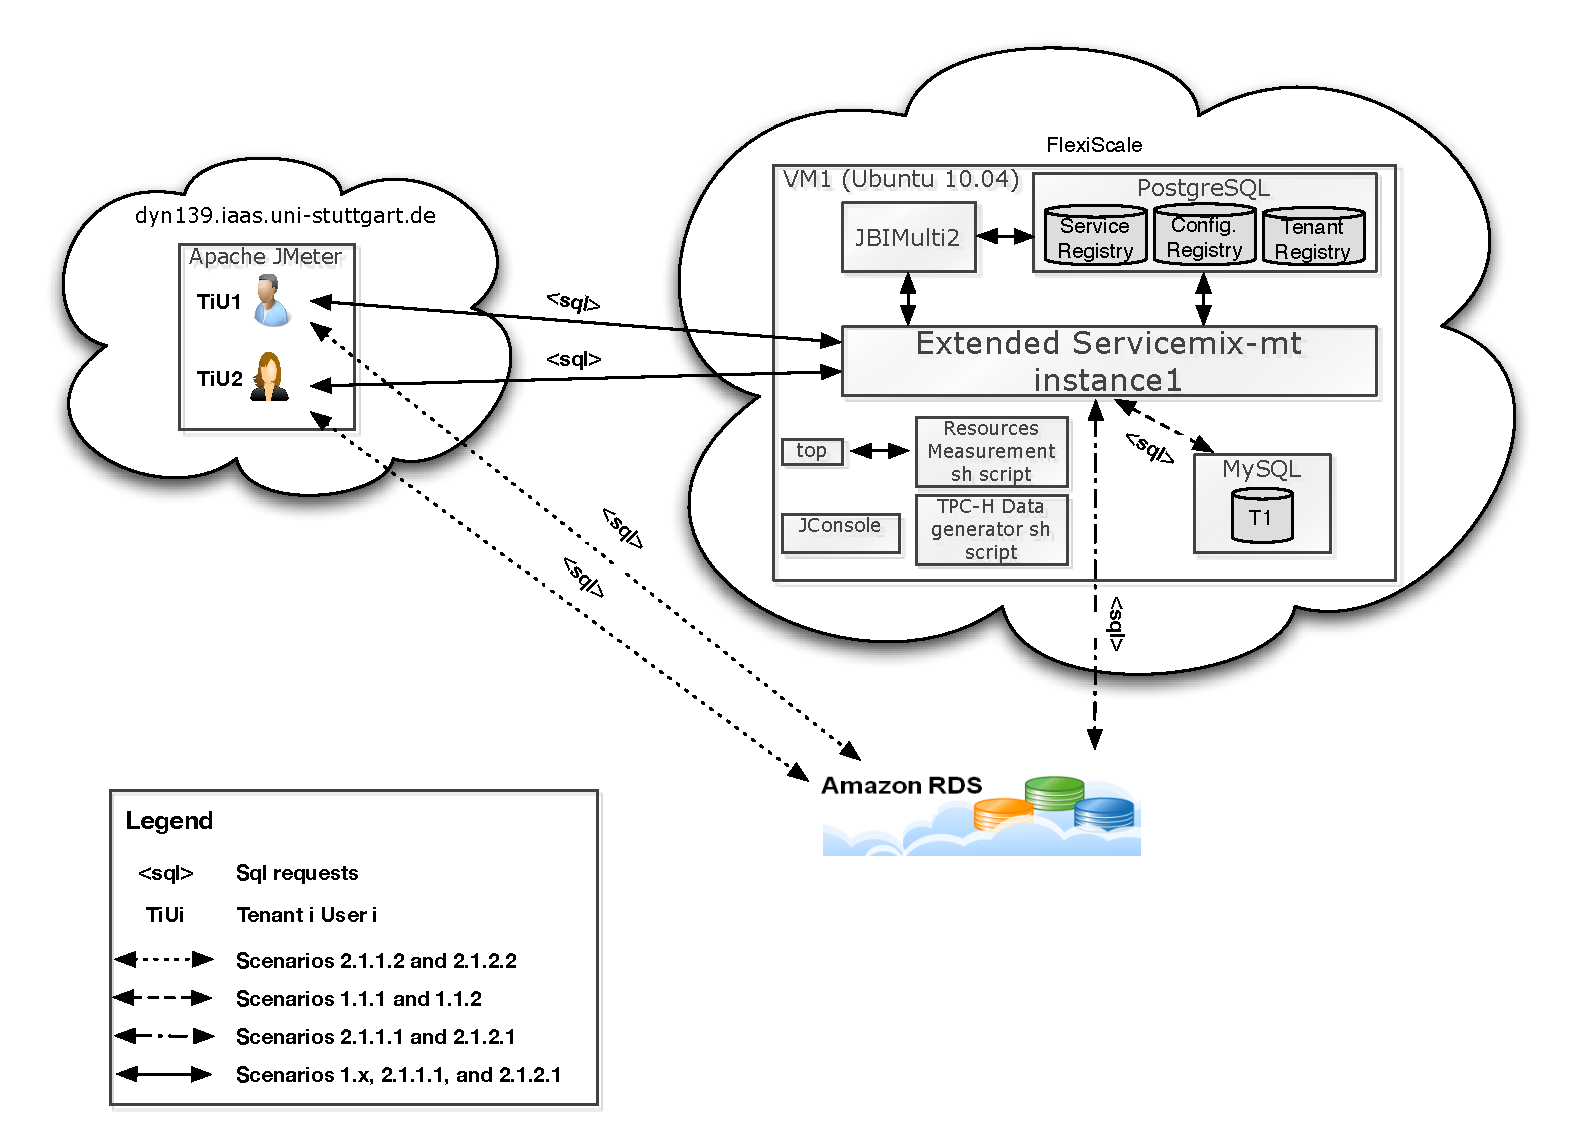
\includegraphics[width=0.7\textwidth, trim=0.0cm 0.0cm 0.0cm 0.0cm, clip]{./gfx/evaluationoverview.pdf}
	\caption[Performance Evaluation Components Overview]{Overview of the components used for the \ac{ESB} performance evaluation. \textbf{Note:} In the evaluation two different monitors are used. For communication the monitoring requires the counting and visualization of the incoming and outgoing requests. For system monitoring, the CPU and Memory usage should be measured.}
	\label{fig:evaluationoverview}
\end{figure}

\FloatBarrier

\FloatBarrier
\section{ESB Performance Evaluation Architecture}
\label{sec:esbevaluationdesign}

% explain the figure
% the evaluation is done for SOAP over HTTP protocols based on a in only message exchange patter, so that we are only masuring how much time does it take to reach the backend service. explain that the dashed lines are because those calls are optional, this means, we divide in to more than one scenario, each scenario testing 1, 2, 4, and 10 endpoints
% for the two instances of servicemix, we provide 10 endpoints in total, and 5in each instance, and the load is divided into the endpoitns. we start with the scenario with 2 endpoints
% explain a little bit the java bench androitlogic driver
% explain that we will use differente messages for the scenarios so that we can decouple them from the scenarios, being able to modify messages independently. results are in a format (I can paste an example of a result from the java benchmark) and then the driver provided by androit to be able to convert it to a csv file
% for concurrent calls between endpoints, we are going to create as many instances of the java benchmark as many endpoints we want to call concurrently by using shell scripting and the & (background task). Explain how many messages we are sending, in factor 2..., and the warmup phase of the esb, so that we ensure that the heap mamory is cleaned (garbage collector)
% system monitoring for the %CPU and %sys memory using the top command and then converting the output data to csv
% jconsole usage for heap measurements
% wireshark just for counting the packages that arrived and pack lost
% to fill the messages, we fill it with random characters and create a <attachment> part in the body

AndroitLogic has developed in their \ac{ESB} Performance Evaluation Round 3 a load generator for different scenarios. After analyzing its main features, we found it suitable for our work, but only if we can include tenant-awareness in the execution. We evaluate the \ac{SOAP} over \ac{HTTP} communication protocol in both native ServiceMix \ac{HTTP} \ac{BC} and in the multi-tenant \ac{HTTP} \ac{BC}. With this we want to evaluate not only the performance of the \ac{ESB} solution we are using in our Cloud infrastructure, but also the penalty caused by the multi-tenant awareness implementation. The \ac{SOAP} over \ac{HTTP} protocol is well known for its usage in Web services. In this evaluation we use as a backend Web service an Echo Service which logs the received requests. For this purpose, we must push the scenarios as close as possible to a real Web service consumption. Therefore, we divide the evaluation system in two virtual machines connected by a network (see Figure \ref{fig:evaluationarchitecture}). 


%%%%%%%%%%%%%%%%%%%%%%%%%%%%%
\begin{figure}[htb]
	\centering
		\includegraphics[width=.95\textwidth, trim=0.0cm 0.0cm 0.0cm 0.0cm, clip]{./gfx/evaluationarchitecture.pdf}
	\caption[ESB Performance Evaluation Architecture]{Architectural overview of the components used for the evaluation of the \ac{ESB} performance. \textbf{Note:} We evaluate only ServiceMix, not the integrated version of ServiceMix with the JBIMulti2 application, in order to be able to perform a direct comparison between the multi-tenant and the non multi-tenant ServiceMix.}
	\label{fig:evaluationarchitecture}
\end{figure}
%%%%%%%%%%%%%%%%%%%%%%%%%%%%%


The virtual machine one hosts the front and backends components: performance benchmark and the Web service. The Web service is deployed in an Apache Tomcat server. The extended performance benchmark is built of the following components: AndroitLogic driver, shell scripts and data converters. The AndroitLogic driver support concurrent users invoking the same endpoint, but not concurrent users between two or more endpoints. Furthermore, it does not support message modification for including tenant information. For this purpose, we have designed the shell scripts which can give support on those two requirements (see Figure \ref{fig:evaluationarchitecture}). In the first place, the shell script modifies or does not modify the message which will be sent by the driver. In the second place, we perform concurrent invocations between endpoints by creating several Unix background tasks of the driver. Each of the tasks results can be dumped in a shared file between the driver instances. However, the results come in non structured format for analysis. Therefore, we convert the data using a converter provided by AndroitLogic \cite{androit2012}. For monitoring the packet lost rate, we will listen on the server's port where the Web service listens with a well known monitoring tool, Wireshark \cite{wireshark}.

We use the virtual machines two and three for hosting the ServiceMix instances. The two instances are used only in non multi-tenant scenarios. For both multi-tenant and non multi-tenant scenarios we must increase the number of concurrent calls to the endpoints. In the requirement we specify scenarios of one, two, four, and ten endpoints. The system performance measurement can be done by system commands. We provide a component which take CPU and Memory measurements and converts its output to structured data for analysis. However, the system memory usage measurements do not give variable percentages over time. The percentage shown is the one associated with the memory consumption of the JVM the \ac{ESB} runs on, which is previously reserved and fixed over time. To get more representative data, we measure the heap consumption of ServiceMix in the JVM using Java Console, which give us a better representation of the variability between the different scenarios (See Figure \ref{fig:evaluationarchitecture}). For monitoring the communication, an instance of Wireshark can also be used, but in our evaluation it is optional.


\FloatBarrier
\clearpage
\section{Evaluation}
\label{sec:evaluation}

In this section we first describe the components we implemented to be able to reuse the existing load performance driver from AndroitLogic \ac{ESB} Performance Round 6 and adapt it to the required multi-tenant scenarios \cite{androit2012}. In Section \ref{sec:evaluationanalysis} we shortly describe the deployment and initialization in the virtual machines under the Flexiscale network \cite{flexiscale} and we evaluate the results obtained from the different scenarios. 

\subsection{ESB Performance Evaluation Benchmark}
% put a figure of the folder skeleton
% explain the androit benchmark (we can put an example of the inputs of the java call)
% explain the endpoint configuration (both multi-tenant and non multi-tenant)
% echo service at the end
% message sample (and explain that we will use the message sample to include the tenant id and user id in the to and from values) so that we can see them in the echo service
% endpoint configuration, for both multi tenant and non multi tenant

AndoitLogic has developed an ESB Performance Benchmark in their Round 6 \cite{androit2012}. Their benchmark evaluates the ServiceMix behavior under different scenarios, which vary in the request message size, number of requests per endpoint, and number of concurrent users per endpoint. Their load generator is included in the \term{org.adroitlogic.toolbox.javabench} package in their Management Toolbox application \cite{androit2012}. They provide an HttpBenchmark and a \term{data to csv format} converter. The former makes \ac{HTTP} POST requests to the specified endpoint URL, and generates performance statistics, e.g. response time, throughput. The latter converts the driver's results to structured data for analysis. We reuse both components, but develop components on top which create several instances of the \term{javabench} to invoke multiple endpoints concurrently. Furthermore, we need to add tenant context information before invoking the driver. The components are implemented in UNIX shell scripts.

%%%%%%%%%%%%%%%%%%%%%%%%%%%%%
\begin{figure}[htb]
	\centering
		\includegraphics[width=.95\textwidth, trim=0.0cm 0.0cm 0.0cm 0.0cm, clip]{./gfx/folderorganizationesbperformance.pdf}
	\caption[ESB Performance Evaluation Package Structure]{Overview of the package used for the evaluation of the \ac{ESB} performance}
	\label{fig:folderarch}
\end{figure}
%%%%%%%%%%%%%%%%%%%%%%%%%%%%%

In Figure \ref{fig:folderarch} we describe the overall structure of our loader package. We define three scenarios: scenario 1 is non multi-tenant aware and with one instance of ServiceMix, scenario 2 is non multi-tenant aware with two instances of ServiceMix, and scenario 3 is multi-tenant aware with 1 instance of ServiceMix \cite{EvalESB}, \cite{EnablingMT}. The \ac{SOAP} messages and the endpoints' URLs are read from \ac{XML} files stored in the \term{scenariox} folder. The messages vary from 500B to 100K. However, in this student thesis we perform the analysis for the 500B and 1K messages' sizes. The main and secondary scripts used in this analysis are located under the main scripts folders and the results generated are stored in the \term{ResultsScenariox} folder. In addition, for the multi-tenant scenarios, the endpoint URL file must also contain the tenant context information, e.g. tenantId and userId. 

For the evaluation scenarios we create using the ServiceMix \ac{HTTP} maven archetype 11 \ac{SU}s. Ten \ac{SU}s contain non multi-tenant endpoint configurations of 10 consumer and 10 providers which support the \ac{SOAP} over \ac{HTTP} communication protocol, while one \ac{SU} is configured to be deployed on the multi-tenant \ac{HTTP} \ac{BC} by 10 tenants, generating 10 tenant-aware endpoints (10 tenant-aware consumer and provider endpoints). The deployment phase is described in Section \ref{sec:evaluationanalysis}.

%%%%%%%%%%%%%%%%%%%%%%%%%%%%%
\lstinputlisting[label={lst:scenarioinvokationi},caption={[ESB Performance Analysis Main Shell Script Invocation] Invocation parameters in the main shell scripts of the benchmark.},basicstyle=\scriptsize]{./gfx/androitinvokation.txt}
%%%%%%%%%%%%%%%%%%%%%%%%%%%%%

For the non multi-tenant scenarios, we specify the needed invocation parameters in Listings \ref{lst:scenarioinvokationi}, \ref{lst:loopinvokation}, and \ref{lst:loopinvokation2}. The non multi-tenant aware shell script takes as one of the input parameters the file path where the \ac{SOAP} message is stored and creates the result scenario file name based on the message size and the running scenario. Furthermore, the endpoints' URLs are retrieved from the endpoint configuration file and the script reads as many URLs as tenants we specify. For supporting concurrent calls between endpoints, we create as many instances of the \term{javabench} as endpoints by running a secondary script, the loop script (see Figure \ref{fig:folderarch}), which is executed as a Linux background task. The scenario is divided in two phases: warm-up and performance test. In the warm-up phase an amount of requests are concurrently sent to the endpoints in order to warm-up the \ac{ESB} and get consistent results, while in the performance test phase we perform the measurements which can be analyzed. In the warmup phase the initial request number is set to 10240 requests. This value is then increased exponentially, and divided by the number of endpoints, as described in the following explanation. The loop script increments exponentially the number of requests and divides it by the number of endpoints in the \ac{ESB}, e.g. during the performance test phase if an initial request number is set to 20, then it sends to each endpoint \begin{math} 20 * 2^i, i = [1,2,3,5,6] \end{math} divided by the number of invoked endpoints in the scenario. The same sequence is applied for the multi-tenant scenario. 

%%%%%%%%%%%%%%%%%%%%%%%%%%%%%
\lstinputlisting[label={lst:loopinvokation},caption={[ESB Performance Analysis Non Multi-tenant Shell Script Invocation]Invocation parameters in the non multi-tenant shell script of the benchmark.},basicstyle=\scriptsize]{./gfx/loopinvokation.txt}
%%%%%%%%%%%%%%%%%%%%%%%%%%%%%

The approaches taken into account for the non multi-tenant scenarios are similar to the multi-tenant scenario, as it is shown in Listing \ref{lst:loopinvokation}. The main difference relies on the need of tenant context information injection before the \ac{SOAP} message is read and sent over \ac{HTTP} concurrently to the tenant-aware endpoints. The concurrent reading of messages leads us to the need of using temporal files to store the messages containing tenant context information. The temporal files are created in the same directory as the requests files, and we modify the content by reading the original request in the loop2 script shown in Listing \ref{lst:loopinvokation2} and using the Linux \term{sed} command to inject the tenant context information read from the endpoints' URL definition file. 

%%%%%%%%%%%%%%%%%%%%%%%%%%%%%
\lstinputlisting[label={lst:loopinvokation2},caption={[ESB Performance Analysis Multi-tenant Shell Script Invocation]Invocation parameters in the multi-tenant shell script of the benchmark.},basicstyle=\scriptsize]{./gfx/loopinvokation2.txt}
%%%%%%%%%%%%%%%%%%%%%%%%%%%%%

With the above approaches we fulfill the requirement of getting the response time and the throughput when invoking and external Web service through an \ac{ESB}. We have also implemented scripts for monitoring the system resources with the \term{top} Linux command and with the Java Console \cite{jconsole}. The former provides data at the system level, e.g. JVM memory consumption, while the latter provides data about the exact amount of JVM resources the ServiceMix process consumes.


\subsection{ESB Performance Evaluation Analysis}
\label{sec:evaluationanalysis}

	In this student thesis we extend and add extra functionality to ServiceMix. Therefore we need to measure its behavior and compare it with the baseline, which is the non multi-tenant version of Apache ServiceMix 4.3.0 \cite{ASM}. In the following sections we describe the systems we use for evaluating the performance of the \ac{ESB}, and we discuss some of the results we obtained. 

	\subsubsection{Deployment and Initialization}
	
	The different scenarios we run in this evaluation must approximate as much as possible to real scenarios. Thus we utilize three Ubuntu 10.04 virtual machines in this evaluation connected by the network in the Flexiscale infrastructure \cite{flexiscale}. One virtual machine hosts the evaluation package and an echo Web service which implements the In-Only \ac{MEP} and is deployed in Tomcat 7.0.23. Wireshark 1.2.7 is installed for monitoring incoming and outgoing requests to and from the echo Web service. In a second and third virtual machine we install one instance of ServiceMix 4.3.0 and the system resources measurement scripts. We have listed in Section \ref{sec:evaluationspecification} a set of multi-tenant and non multi-tenant scenarios. For the non multi-tenant scenarios we have deployed in the ServiceMix \term{deploy} directory a \ac{SA} containing the configuration of 10 consumer and 10 provider endpoints. For the multi-tenant scenarios we performed the operations described in Section \ref{sec:multitenanttest} and deploy through JBIMulti2 10 tenant-aware consumer and 10 tenant-aware provider endpoints. Both tenant-aware and non tenant-aware endpoints must be specified in the endpoint file the extended driver reads for sending the \ac{SOAP} requests.
	
	
	\subsubsection{Evaluation Analysis}
	
	%%%%%%%%%%%%%%%%%%%%%%%%%%%%%
	\begin{figure}[htb]
		\centering
			\includegraphics[clip, scale=0.5]{./gfx/response1K.pdf}
		\caption[ESB Performance Evaluation Response time for 1KB Messages]{Response time of the different scenarios for 1KB \ac{SOAP} over \ac{HTTP} requests \cite{EvalESB}.}
		\label{fig:responsetime}
	\end{figure}
	%%%%%%%%%%%%%%%%%%%%%%%%%%%%%
	
	The numerical values obtained from the communication driver are distributed per endpoint. Therefore, we make the average between the endpoints for each set of sent requests. The latency when increasing the number of endpoints in the system increases between 25\% and 45\% for concurrent requests sent to 2, 4 and 10 endpoints (see Figure \ref{fig:responsetime}). We can see that our extended version declines the original ServiceMix's performance approximately 30\% \cite{EvalESB}. Furthermore, we can observe that the response time for the different multi-tenant scenarios does not increase proportional to the number of tenants, but shows a better performance per endpoint. When distributing the requests between two ServiceMix instances we have observed that the response time is substantially reduced when increasing the number of endpoints.	
	
	%%%%%%%%%%%%%%%%%%%%%%%%%%%%%
	\begin{figure}[htb]
		\centering
			\includegraphics[clip, scale=0.7]{./gfx/evaluation_throughput.pdf}
		\caption[ESB Performance Evaluation Throughput for 1KB Messages]{Throughput of the different scenarios for 1KB \ac{SOAP} over \ac{HTTP} requests \cite{EvalESB}.}
		\label{fig:evaluationthroughput}
	\end{figure}
	%%%%%%%%%%%%%%%%%%%%%%%%%%%%%	
		
	When measuring the throughput, the analysis took us to the same deduction we discussed above. When the number of endpoints decreases, we can observe a bigger gap between the native and the extended version of ServiceMix. As we increase the number of endpoints, e.g. 10 endpoints, we can see that the gap between approaches is exponentially narrowed (see Figure \ref{fig:evaluationthroughput}).  
	
	%%%%%%%%%%%%%%%%%%%%%%%%%%%%%
	\begin{figure}[htb]
		\centering
			\includegraphics[clip, scale=0.5]{./gfx/evaluation_cpu.pdf}
		\caption[ESB Performance Evaluation CPU Consumption]{Overview of the CPU consumption over the different scenarios \cite{EvalESB}.}
		\label{fig:evaluationcpu}
	\end{figure}
	%%%%%%%%%%%%%%%%%%%%%%%%%%%%%
	
	Finally, we have analyzed the CPU consumption of the process running the ServiceMix instance. We can observe in the average CPU consumption that there is a gap between both multi-tenant and non multi-tenant scenarios which increases when the number of endpoints increases. However, when increasing the number of endpoints the average CPU consumption stabilizes and maintains close to a constant value. The maximum CPU consumption values decreases in the non multi-tenant scenarios when increasing the number of endpoints, while for the multi-tenant scenario it linearly increases from two endpoints. In the 4 or 10 endpoints scenarios, the maximum CPU consumption difference between the native and the extended approaches are between 250\% and 320\% approximately (see Figure \ref{fig:evaluationcpu}).

The tenant authentication procedure demands a greater number of resources when parsing the \ac{SOAP} headers and the \ac{XML} data from the tenant context file. However, this decline caused by the implemented authentication procedure and the marshaling of tenant context information within the process is much lower that the decline caused by establishing a connection with an external database system and retrieving the tenant context information from an external source to the process.  
	
	



